\documentclass[aps, pre, onecolumn, nofootinbib, notitlepage, groupedaddress, amsfonts, amssymb, amsmath]{revtex4-1}
%%%%%%begin preamble
\usepackage[hmargin=1in, vmargin=1in]{geometry} % Margins
\usepackage{hyperref}
\usepackage{url}
\usepackage{natbib}
\setlength{\bibsep}{0pt plus 0.3ex}
\usepackage{graphicx}
%\usepackage{pdfpages} % breaks with aastex6
\usepackage{import}
\usepackage{wrapfig}

\usepackage{xcolor}
\hypersetup{
  colorlinks   = true,
  %citecolor    = blue
  citecolor    = gray
  % gray is not being found!?!
  % gray is found if pdfpages is used... crap.
  %citecolor    = grey
  %citecolor    = Gray
}

%Copy+pasted from aastex.
\newcommand\aj{\ref@jnl{AJ}}%        % Astronomical Journal 
\newcommand\araa{\ref@jnl{ARA\&A}}%  % Annual Review of Astron and Astrophys 
\renewcommand\apj{ApJ}%    % Astrophysical Journal ++
\newcommand\apjl{ApJL}     % Astrophysical Journal, Letters 
\newcommand\prf{Phys.~Rev.~Fluids}     % Astrophysical Journal, Letters 
\newcommand\apjs{\ref@jnl{ApJS}}%    % Astrophysical Journal, Supplement 
\renewcommand\ao{\ref@jnl{ApOpt}}%   % Applied Optics ++
\newcommand\apss{\ref@jnl{Ap\&SS}}%  % Astrophysics and Space Science 
\newcommand\aap{\ref@jnl{A\&A}}%     % Astronomy and Astrophysics 
\newcommand\aapr{\ref@jnl{A\&A~Rv}}%  % Astronomy and Astrophysics Reviews 
\newcommand\aaps{\ref@jnl{A\&AS}}%    % Astronomy and Astrophysics, Supplement 
\newcommand\azh{\ref@jnl{AZh}}%       % Astronomicheskii Zhurnal 
\newcommand\baas{\ref@jnl{BAAS}}%     % Bulletin of the AAS 
\newcommand\icarus{\ref@jnl{Icarus}}% % Icarus
\newcommand\jrasc{\ref@jnl{JRASC}}%   % Journal of the RAS of Canada 
\newcommand\memras{\ref@jnl{MmRAS}}%  % Memoirs of the RAS 
\newcommand\mnras{MNRAS}%   % Monthly Notices of the RAS 
\renewcommand\pra{\ref@jnl{PhRvA}}% % Physical Review A: General Physics ++
\renewcommand\prb{\ref@jnl{PhRvB}}% % Physical Review B: Solid State ++
\renewcommand\prc{\ref@jnl{PhRvC}}% % Physical Review C ++
\renewcommand\prd{\ref@jnl{PhRvD}}% % Physical Review D ++
\renewcommand\pre{\ref@jnl{PhRvE}}% % Physical Review E ++
\renewcommand\prl{\ref@jnl{PhRvL}}% % Physical Review Letters 
\newcommand\pasp{\ref@jnl{PASP}}%     % Publications of the ASP 
\newcommand\pasj{\ref@jnl{PASJ}}%     % Publications of the ASJ 
\newcommand\qjras{\ref@jnl{QJRAS}}%   % Quarterly Journal of the RAS 
\newcommand\skytel{\ref@jnl{S\&T}}%   % Sky and Telescope 
\newcommand\solphys{\ref@jnl{SoPh}}% % Solar Physics 
\newcommand\sovast{\ref@jnl{Soviet~Ast.}}% % Soviet Astronomy 
\newcommand\ssr{SSRv}% % Space Science Reviews 
\newcommand\zap{\ref@jnl{ZA}}%       % Zeitschrift fuer Astrophysik 
\renewcommand\nat{\ref@jnl{Nature}}%  % Nature 
\newcommand\iaucirc{\ref@jnl{IAUC}}% % IAU Cirulars 
\newcommand\aplett{\ref@jnl{Astrophys.~Lett.}}%  % Astrophysics Letters 
\newcommand\apspr{\ref@jnl{Astrophys.~Space~Phys.~Res.}}% % Astrophysics Space Physics Research 
\newcommand\bain{\ref@jnl{BAN}}% % Bulletin Astronomical Institute of the Netherlands 
\newcommand\fcp{\ref@jnl{FCPh}}%   % Fundamental Cosmic Physics 
\newcommand\gca{\ref@jnl{GeoCoA}}% % Geochimica Cosmochimica Acta 
\newcommand\grl{\ref@jnl{Geophys.~Res.~Lett.}}%  % Geophysics Research Letters 
\renewcommand\jcp{\ref@jnl{JChPh}}%     % Journal of Chemical Physics 
\newcommand\jgr{\ref@jnl{J.~Geophys.~Res.}}%     % Journal of Geophysics Research 
\newcommand\jqsrt{\ref@jnl{JQSRT}}%   % Journal of Quantitiative Spectroscopy and Radiative Trasfer 
\newcommand\memsai{\ref@jnl{MmSAI}}% % Mem. Societa Astronomica Italiana 
\newcommand\nphysa{\ref@jnl{NuPhA}}%     % Nuclear Physics A 
\newcommand\physrep{\ref@jnl{PhR}}%       % Physics Reports 
\newcommand\physscr{\ref@jnl{PhyS}}%        % Physica Scripta 
\newcommand\planss{\ref@jnl{Planet.~Space~Sci.}}%  % Planetary Space Science 
\newcommand\procspie{\ref@jnl{Proc.~SPIE}}%      % Proceedings of the SPIE 

\newcommand\actaa{\ref@jnl{AcA}}%  % Acta Astronomica
\newcommand\caa{\ref@jnl{ChA\&A}}%  % Chinese Astronomy and Astrophysics

\setcounter{tocdepth}{2}
%% headers
\usepackage{fancyhdr}
\pagestyle{fancy}
\fancyhf{} % sets both header and footer to nothing
\lhead{Evan Anders---Research Statement}
\rhead{Stanford University, Stanford Science Fellows}
\cfoot{\footnotesize{\thepage}}
%\pagestyle{empty}
%\pagenumbering{gobble}
%\renewcommand*{\thefootnote}{\fnsymbol{footnote}}

\renewcommand{\vec}{\ensuremath{\boldsymbol}}
\newcommand{\dedalus}{\href{http://dedalus-project.org}{Dedalus}}
\newcommand{\del}{\ensuremath{\vec{\nabla}}}
\newcommand{\scrS}{\ensuremath{\mathcal{S}}}

\newcommand{\nosection}[1]{%
  \refstepcounter{section}%
  \addcontentsline{toc}{section}{\protect\numberline{\thesection}#1}%
  \markright{#1}}
\newcommand{\nosubsection}[1]{%
  \refstepcounter{subsection}%
  \addcontentsline{toc}{subsection}{\protect\numberline{\thesubsection}#1}%
  \markright{#1}}

%\usepackage{atbegshi}
%%%%%%end preamble


\begin{document}
\section*{Motivation and Research Problem}
\vspace{-13pt}
Stars enable most studies in astrophysics.
Stars are the progenitors of exotic objects like black holes and detecting exoplanets or sampling the composition of interstellar space are some of the many uses of measured starlight.
In addition to their importance to diverse astrophysical subdisciplines, stars themselves are fascinating experiments where fluid dynamical processes occur at extreme parameters.
Asteroseismology is a relatively new field which measures sound and gravity waves at the surface of stars and, akin to seismic measurements on the Earth, traces the paths of those waves through the depths of the star to learn about its interior structure.
This technique enables the precise determination of age, mass, and radius of many stars, particularly stars like the Sun.
Models of stellar interiors are essential for the interpretation of asteroseismic and helioseismic data.
Sun-like stars exhibit highly turbulent near-surface convective regions, but state-of-the-art codes which generate stellar structure models used in asteroseismology rely on decades-old, one-dimensional (1D) parameterizations of convection.
These parameterizations, and most convective theory, predict that ``giant cells'' which are characterized by large-scale horizontal motions should be driven in the convection zone of Sun-like stars, but high resolution observations of the Sun have been unable to detect these giant cells.
The absence of these flows has called into question our most fundamental understanding of the nature of convection in stars, a problem widely referred to as the ``Solar Convective Conundrum.''
Sorting out this Convective Conundrum is crucial for having confidence in present and future asteroseismic results, particularly in the modern age where asteroseismic measurements are being performed for more than $10^4$ stars in our galaxy.

Modern simulations of convection often reproduce the convective flows at the stellar surface quite reliably, but the deep convective motions, where giant cells would be driven, are still poorly constrained and understood.
My research aims to help solve the Convective Conundrum by using analytical and numerical techniques to study simplified models of stellar convection which can be extrapolated to gain insight into the nature of convection in the highly stratified, rotating, magnetized context of stellar convection.
During my time at Stanford, I will conduct a series of studies which will span from the smallest to the largest scales present in stellar convection.
I will use the understanding gained in detailed, small-scale studies of deep convection to inform the interpretation of large-scale global studies which model a full stellar convection zone.
While I draw my inspiration from problems facing the solar and stellar community, similar flow processes may be important in the atmospheres and cores of planets like Jupiter and the Earth. 


\vspace{-16pt}
\section*{Research Plan}
\vspace{-13pt}
\paragraph*{The smallest convective scales: individual downflows}
\begin{wrapfigure}{r}{0.22\textwidth}
	\begin{center}
	\vspace{-25pt}
    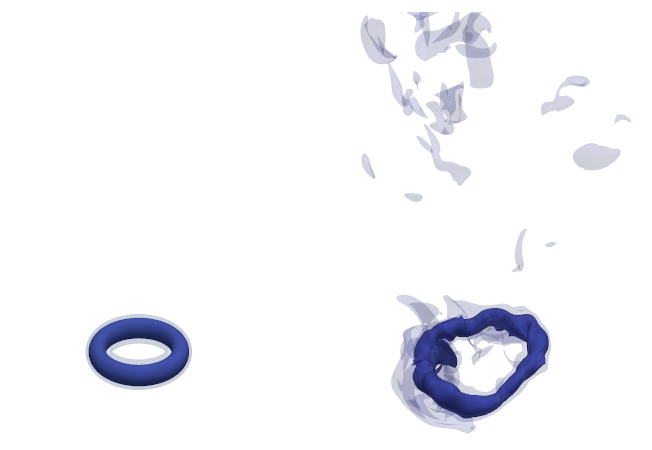
\includegraphics[width=0.21\textwidth]{./figs/thermals_comparison.png}
	\vspace{-20pt}
	\end{center}
    \caption{
	3D visualizations of entropy perturbations in the downward-propagating reference frame of evolved laminar (left) and turbulent (right) thermals.
	\label{fig:thermals_comparison} }
	\vspace{-22pt}
\end{wrapfigure}
Convection at the Sun's surface exhibits a fundamental property of convection in stratified atmospheres: broad, slow upwellings and intense, fast downflows.
It is hypothesized that these downflows may be so powerful that they alone transport the Sun's luminosity in the deep convection zone.
These downflows would exist alongside mass-conserving upflows which exhibit negligible energy transport.
This ``entropy rain'' hypothesis, first suggested by \citet{spruit1997}, is gaining traction in recent simulations \cite{kapyla&all2017} and theoretical work \citep{brandenburg2016}, and could explain the absence of giant cells in observations \citep{hanasoge&all2015}.
These downflows may turbulently break up into distinct pieces as they fall and these individual downflow pieces can be modeled as ``thermals.''
Thermals are regions of cold fluid which accelerate due to buoyancy forces and shape themselves into vortex rings; evolved thermals are visualized in Fig. \ref{fig:thermals_comparison}, and thermals are studied extensively in Earth's atmosphere \citep{lecoanet&jeevanjee2019}.

As a Stanford fellow, I will build upon my previous study of thermals \citep{andersLB2019} to continue to learn whether entropy rain is the cause of the convective conundrum.
Stellar convective flows are highly turbulent and experience global rotation and strong magnetic fields, and it is possible that these effects can ``evaporate'' entropy rain.
I will determine whether rotation, magnetism, and turbulence can prevent downflows from successfully transiting the convection zone.

\paragraph*{Intermediate-scale interactions at the radiative-convective boundary}
In Sun-like stars, the turbulent convection zone lies above a stably stratified ``radiative zone'' where radiation effectively carries the stellar luminosity.
In the Sun, the radiative-convective boundary (RCB) is characterized by a transition from moderate instability to strong stability, and coincides with a region of intense shear in the Sun's radial velocity profile called the tachocline.
The tachocline is thought to be a crucial driver of the Sun's magnetic dynamo.
If stellar downflows are truly important, as the entropy rain hypothesis suggests, it is critical to learn how downflows pump angular momentum and magnetism into the RCB to better understand how the solar dynamo is driven, and how the tachocline was established.
%Measurements suggest that the RCB is thin \citep{basu1997}, but many modern simulations produce RCBs which are up to an order of magnitude thicker than the solar one \citep{hotta2017}.
%This suggests that many simulations are studying angular momentum and magnetic field pumping mechanisms in the wrong regime of ``stiffness'' of the RCB \citep{couston&all2017}.

During my time at Stanford, I will study how an ensemble of downflows interacts with a solar-like RCB.
These studies will be conducted in parameter regimes where downflows can transit the convection zone, as determined by my proposed single-downflow studies.
I will simulate localized, rotating magnetoconvection and study convective pumping mechanisms into a solar-like RCB.

\begin{wrapfigure}{r}{0.22\textwidth}
	\begin{center}
	\vspace{-22pt}
    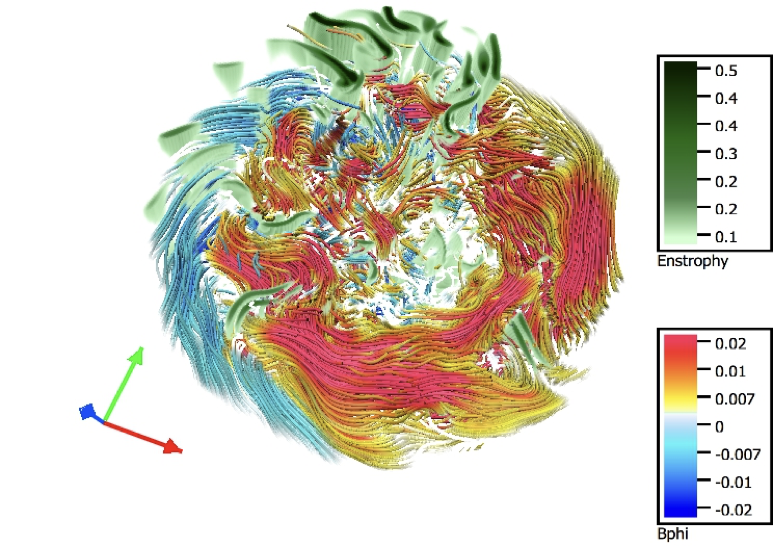
\includegraphics[width=0.21\textwidth]{./figs/mdwarf.png}
	\vspace{-16pt}
	\end{center}
    \caption{A volume rendering of a global dynamo simulation in Dedalus.
	Enstrophy, or the magnitude of vorticity, is shown in green.
	Red and blue lines denote the magnitude and direction of azimuthal magnetic field.
	\label{fig:mdwarf} }
	\vspace{-11pt}
\end{wrapfigure}
\paragraph*{Global convection simulations: dynamics in relaxed atmospheres}
Recently, researchers have sought mechanisms for coupling 1D stellar models with fully convective, three-dimensional (3D) global simulations due to deficiences in decades-old 1D convective parameterizations \citep{bohm-vitense1958}.
The coupling of near-surface simulations with 1D models was recently done successfully \citep{jorgensen&weiss2019}.
However, this coupling was performed \emph{after} the simulations had been computed, not at runtime, and such a coupling is not yet available for deep convective motions, where parameterizations assume giant cells are driven.
One reason that this coupling does not yet occur at runtime is because simulations of deep convection have system equilibration timescales which are very disparate from the characteristic timescales of convective overturn..
Evolving through these equilibration timescales is time ``wasted'' waiting for convergence of the atmospheric structure and mean flows, but this expense can be minimized using clever numerical techniques.

During my time at Stanford, I will design a generalized public module which can accelerate mean profiles and flows in global simulations.
This module will read in statistical measures from unequilibrated convective simulations and output the properly equilibrated mean state.
I previously developed such a tool in cartesian simulations \citep{anders&all2018}, and will extend this to global simulations like the one shown in Fig.~\ref{fig:mdwarf}.
The large-scale structures in Fig.~\ref{fig:mdwarf} arise quickly, but the equilibration and saturation of these structures take so long that they cannot be feasibly simulated in turbulent regimes.
This tool will benefit numericists across diverse research fields, such as those who study general circulation models (GCMs) in the atmospheres of the Earth and exoplanets or modelers of dynamo processes in planetary cores and stellar atmospheres.
Once completed, I will use this tool in my own research to study equilibrated global simulations of solar-like stars in the regimes which my small- and medium-scale simulations show that downflows can survive and play important dynamical roles.


\vspace{-15pt}
\section*{How Stanford enables these accomplishments}
\vspace{-13pt}
Stanford is the perfect location for carrying out this work due to the opportunities available for interdisciplinary collaboration between astrophysicists, geophysical fluid dynamicists, applied mathematicians, and experts in turbulence.
The most natural collaborator on this work proposed here is Prof.~Tom Abel of Stanford's physics department and the SLAC National Accelerator Laboratory; his expertise in astrophysical fluid dynamics and scientific visualization, as well as his broad interest on astrophysical topics would make him an excellent mentor as I tackle these problems and grow as a researcher.
From Prof.~Abel's group, I would collaborate with the numerous experts in Stanford's Physics department, such as Prof.~Petrosian, who has recently studied the hydrodynamics of solar flares and Prof.~Wagoner, who has studied waves in astrophysical accretion disks.
I would collaborate with Stanford's experts on atmospheric and oceanic processes in the School of Earth, Energy \& Environmental Sciences department, such as Profs.~Sheshadri and Thomas; many fundamental fluid dynamical processes present in stars play roles in the Earth's atmospheres and oceans, which they study.
Furthermore, experts in Stanford's Mathematics departments with experience in fluid flows (e.g., Profs.~Ryzhik and Tokieda) and numerical methods (e..g, Prof.~Kazeev) will be valuable collaborators while I ensure that my numerical methodologies and theories are sound.
Finally, Stanford's Center for Turbulence Research, which houses many experts on turbulent fluid dynamics such as Prof.~Javier Jim\'{e}nez, will be an invaluable resource as I carry out my research plan.
I will carry out my simulations using the Dedalus code \citep{burns&all2019}, which I have used throughout my graduate career, and the computational resources available through Stanford's Research Computing Center, like the Sherlock HPC cluster.

The Stanford Science Fellows program would give me the freedom to study these ambitious problems in astrophysical fluid dynamics.
The projects proposed here seek to understand stellar convection from small to global scales and build naturally upon my PhD research.
These projects help solve exciting problems in stellar structure with applications in numerous astrophysical subdisciplines.
I look forward to the opportunity to create cross-disciplinary collaborations and carry on Stanford's excellent research tradition while making lasting contributions which help solve the Convective Conundrum and other fascinating problems. 

\bibliographystyle{yahapj}
\bibliography{biblio}
\end{document}
